
% This LaTeX was auto-generated from an M-file by MATLAB.
% To make changes, update the M-file and republish this document.

\documentclass{article}
\usepackage{graphicx}
\usepackage{color}
\usepackage{listings}
\usepackage[framed]{mcode}
\usepackage{fullpage}
\usepackage{hyperref}
\usepackage{amsmath}

\definecolor{lightgray}{gray}{0.5}
\setlength{\parindent}{0pt}

\begin{document}

    
    
%\section*{}

\begin{par}

\title{BE 521 - Homework X\\{\normalsize Spring 2015}}
\author{Mike Lautman}
\date{\today}
\maketitle

\end{par}
\begin{par}

\section*{1. Unit Activity}
\subsection*{1.1 1.1 IEEG portal spikes}
\includegraphics[width=400]{./img/three_peaks_IEEg.png}.

\end{par}
\begin{lstlisting}
clear; clc; clf; close all;
session = IEEGSession('I521_A0001_D001', 'mlautman', 'mla_ieeglogin.bin');

disp('1.2 session')
disp(session)

disp('1.3 sample_rate')
data=session.data;
sample_rate = data.sampleRate;
disp(sample_rate)

disp('1.4 recording_length')
recording_length= data.channels(1).getNrSamples;
recording_length_s = recording_length/sample_rate;
disp(recording_length_s)


disp('1.5a same window')
s_s = 8.75;
e_s = s_s + .5;
s = max(round(s_s*sample_rate), 1);
e = min(round(e_s*sample_rate), recording_length);
vals = data.getvalues(s:e,1);
figure(1);
plot(...
    (s:e)./data.sampleRate, ...
    vals, ...
    'color', ...
    'b' ...
);
xlim([s_s, e_s]);
ylabel('Voltage (mV)', 'FontSize',10,'FontWeight','bold');
xlabel('Time (S)', 'FontSize',10,'FontWeight','bold');
title('Three spikes from IEEG dataset I521\_A0001\_D001', 'FontSize',12,'FontWeight','bold');
print -dpng ./img/three_spikes_matlab

disp('1.5b spikes')
disp('we define a spike as a locally convex region where the local maxima is greater than 5*std from the mean.')
figure(2)
v_ave = mean(vals);
v_std = std(vals);
vals_spikes = (vals - v_ave > 5 * v_std) .* vals;
[pks,locs] = findpeaks(vals_spikes);
hold on
plot(...
    (s:e)./data.sampleRate, ...
    vals, ...
    'color', ...
    'b' ...
);
plot((s + locs)/sample_rate,pks, 'x', 'color','r');

xlim([s_s, e_s]);
ylabel('Voltage (mV)', 'FontSize',10,'FontWeight','bold');
xlabel('Time (S)', 'FontSize',10,'FontWeight','bold');
title('Three peaks from IEEG dataset I521\_A0001\_D001', 'FontSize',12,'FontWeight','bold');
print -dpng ./img/three_peaks_matlab

disp('1.5b total spikes in recording')
vals_all = data.getvalues(1:recording_length,1);
v_all_ave = mean(vals_all);
v_all_std = std(vals_all);
vals_all_spikes = (vals_all - v_all_ave > 5 * v_all_std) .* vals_all;
[pks_all,locs_all] = findpeaks(vals_all_spikes);
disp(length(pks_all))
\end{lstlisting}

\color{lightgray} \begin{lstlisting}IEEGSETUP: Adding 'ieeg-matlab.jar' to dynamic classpath
Warning: Objects
of
edu/upenn/cis/db/mefview/services/TimeSeriesIdAndDCheck
class exist -
not clearing
java 
IEEGSETUP: Found log4j on Java classpath.
URL: https://www.ieeg.org/services
Client user: mlautman
Client password: ****
1.2 session
  <a href="matlab:help('IEEGSession')">IEEGSession</a>:

      server: 'ieeg.org'
    userName: 'mlautman'
        data: [1x1 IEEGDataset]

  <a href="matlab:methods(IEEGSession)">Methods</a>, <a href="matlab:IEEGObject.openPortalSite()">main.ieeg.org</a>

1.3 sample_rate
       32051

1.4 recording_length
    10

1.5a same window
1.5b spikes
we define a spike as a locally convex region where the local maxima is greater than 5*std from the mean.
1.5b total spikes in recording
    42

\end{lstlisting} \color{black}


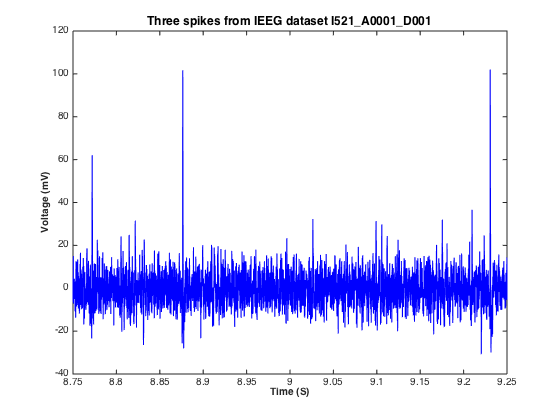
\includegraphics [width=4in]{main_01.png}


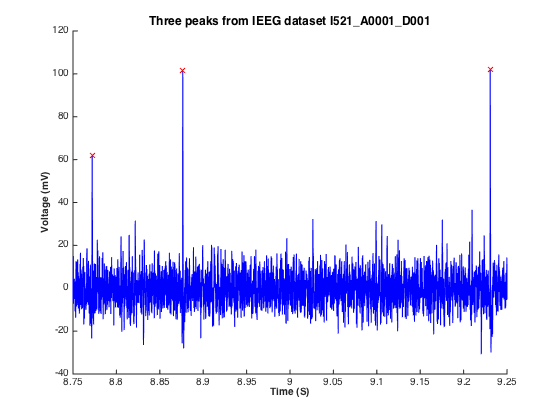
\includegraphics [width=4in]{main_02.png}



\end{document}
    
